\documentclass{astroedu-lab}

\begin{document}

\pagestyle{plain}

\begin{problem}{\huge Лабораторная работа 1.3.1\\\\Определение модуля Юнга\\\\Выполнил Жданов Елисей Б01-205}

\section{Цель работы:}

1)Экспериментально получить зависимость между напряжением и деформацией (закон Гука) для простейшего напряженного состояния упругих тел - одноосного растяжения.

2)По результатам измерений вычислить модуль Юнга.

\section{Оборудование:}

В работе используются: Прибор Лермантова, проволока из исследуемого материала, зритетьная труба со шкалой, набор грузов, микрометр, 2-х метровая линейка.

\newpage

\section{Теоретическая справка:}

Связь между удлинением проволоки $\Delta \mathrm{l}$ и силой Р, вызывающей это удлинение, выражается законом Гука:

$$
\boxed{\frac{P}{S}=E \frac{\Delta l}{L}}
$$

Для определения модуля Юнга используется прибор Лермантова, схема которого изображена на рис. 1. Верхний конец проволоки \textbf{П}, изготовленной из исследуемого материала, прикреплен к консоли \textbf{К}, а нижний - к цилиндру, которым оканчивается шарнирный кронштейн \textbf{Ш}. На этот же цилиндр опирается рычаг \textbf{r}, связанный с зеркальцем \textbf{3}. Таким образом, удлинение проволоки можно измерить по углу поворота зеркальца.

\begin{wrapfigure}{r}{0.4\textwidth}
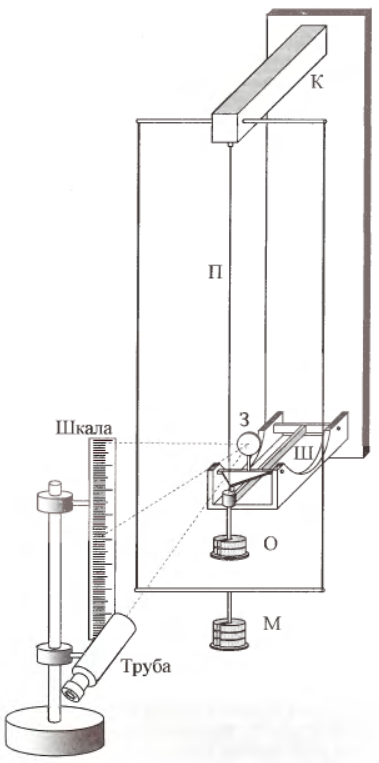
\includegraphics[width=0.4\textwidth]{pribor.png}
\caption{}
\label{ris:image}
\end{wrapfigure}.

Натяжение проволоки можно менять, перекладывая грузы с площадки \textbf{М} на площадку \textbf{О} и наоборот. Такая система позволяет исключить влияние деформации кронштейна \textbf{K} на точность измерений, так как нагрузка на нем все время остается постоянной.

При проведении эксперимента следует иметь в виду, что проволока \textbf{П} при отсутствии нагрузки всегда несколько изогнута, что не может не сказаться на результатах, особенно при небольших нагрузках. Проволока вначале не столько растягивается, сколько распрямляется.

\section{Измерения и обработка:}

1) Убедимся, что установка откалибравана. Выведем искомую формулу.

Угловой наклон зеркала:

\begin{equation}
	\Delta \alpha \approx \frac{\Delta n}{2 h}
\end{equation}

Удлинение проволки


\begin{equation}
	\boxed{\Delta l = \frac{\Delta n \cdot r}{2 h}}
\end{equation}

Задам $\Delta n$ как $n_i - n_0$; $n_0 = 11$ см

2) Использую заданный диаметр проволки($d = 0.73$ мм) для нахождения площади сечения

\begin{equation}
	S = \frac{\pi d^2}{4} = 0.42 \text{ мм}^2
\end{equation}

3) Длину проволки замеряю линейкой

\begin{equation}
	L = (179 \pm 0.5) \text{ см}
\end{equation}

Запишу также остальные замеры

\begin{equation}
	h = (137 \pm 0.5) \text{ см}
\end{equation}

\begin{equation}
	r = 1.3 \text{ см}
\end{equation}

4) Предельная масса для замера

\begin{equation}
	M_{max} = 0.3 \sigma S \approx 10 \text{ кг}
\end{equation}

Имеющиеся грузы имеют суммарную массу порядка 3 кг. Это сильно меньше предела, и как впоследствии будет видно, не способно необратимо изменить длину проволки.

5) Построю таблицу, которую постепенно буду заполнять новыми данными

\begin{center}
\begin{tabular}[t]{|c|l|l|l|l|l|l|l|l|c|}
\hline
& m, кг & P, Н & \multicolumn{6}{|c|}{n, см/$\Delta n$} & $\overline{n}$, см \\
\hline
&&& $\downarrow$ & $\uparrow$ & $\downarrow$ & $\uparrow$ & $\downarrow$ & $\uparrow$ & \\
\hline
1  & +0		& 0 	& 11.2 & 11.2 & 11.2 & 11.1 & 11.1 & 11.5 & $(11.22 \pm 0.06)$ \\
2  & +245.8 & 2.41  & 12.5 & 12.5 & 12.6 & 12.5 & 12.6 & 12.7 & $(12.57 \pm 0.03)$ \\
3  & +246.1 & 4.83  & 13.7 & 13.4 & 13.7 & 13.8 & 13.8 & 13.9 & $(13.72 \pm 0.07)$ \\
4  & +245.5 & 7.23  & 15.0 & 14.6 & 14.9 & 15.0 & 15.0 & 15.3 & $(14.97 \pm 0.09)$ \\
5  & +245.7 & 9.64  & 16.2 & 15.9 & 16.2 & 16.2 & 16.2 & 16.4 & $(16.18 \pm 0.07)$ \\
6  & +246.1 & 12.06 & 17.2 & 17.1 & 17.3 & 17.3 & 17.4 & 17.4 & $(17.28 \pm 0.05)$ \\
7  & +245.6 & 14.47 & 18.3 & 18.3 & 18.5 & 18.5 & 18.6 & 18.6 & $(18.47 \pm 0.06)$ \\
8  & +245.6 & 16.88 & 19.5 & 19.5 & 19.8 & 19.7 & 19.8 & 19.8 & $(19.68 \pm 0.06)$ \\
9 & +245.2  & 19.28 & 20.7 & 20.7 & 20.9 & 20.9 & 20.9 & 20.9 & $(20.83 \pm 0.04)$ \\
10 & +245.7 & 21.69 & 21.9 & 21.9 & 22.0 & 22.0 & 22.1 & 22.1 & $(22.00 \pm 0.04)$ \\
\hline
\end{tabular}
\end{center}

Погрешность $\overline{n}$ является среднеквадратичным отклонением, то есть $\sigma$

Задам $\Delta n$ как $n_i - n_0$; $n_0 = 11.22$ см

Построю итоговую таблицу

\begin{center}
\begin{tabular}[t]{|c|c|c|c|l|l|}
\hline
& $\overline{n}$ & $\overline{\Delta n}$ & $\overline{\Delta l}$, мм & E, 100 ГПа & 1/P  \\
\hline
1  & $(11.22 \pm 0.06)$ & $(0.00  \pm 0.06)$ & $(0.000 \pm 0.003)$ & 0 & inf \\
2  & $(12.57 \pm 0.03)$ & $(1.35  \pm 0.03)$ & $(0.064 \pm 0.002)$ & $(1.61 \pm 0.05)$ & 0.4149 \\
3  & $(13.72 \pm 0.07)$ & $(2.50  \pm 0.07)$ & $(0.118 \pm 0.004)$ & $(1.74 \pm 0.06)$ & 0.2070 \\
4  & $(14.97 \pm 0.09)$ & $(3.75  \pm 0.09)$ & $(0.177 \pm 0.005)$ & $(1.74 \pm 0.05)$ & 0.1383 \\
5  & $(16.18 \pm 0.07)$ & $(4.96  \pm 0.07)$ & $(0.235 \pm 0.004)$ & $(1.75 \pm 0.04)$ & 0.1037 \\
6  & $(17.28 \pm 0.05)$ & $(6.06  \pm 0.05)$ & $(0.286 \pm 0.003)$ & $(1.80 \pm 0.02)$ & 0.0829 \\
7  & $(18.47 \pm 0.06)$ & $(7.25  \pm 0.06)$ & $(0.343 \pm 0.003)$ & $(1.80 \pm 0.02)$ & 0.0691 \\
8  & $(19.68 \pm 0.06)$ & $(8.46  \pm 0.06)$ & $(0.400 \pm 0.004)$ & $(1.80 \pm 0.02)$ & 0.0592 \\
9  & $(20.83 \pm 0.04)$ & $(9.61  \pm 0.04)$ & $(0.454 \pm 0.003)$ & $(1.81 \pm 0.02)$ & 0.0519 \\
10 & $(22.00 \pm 0.04)$ & $(10.78 \pm 0.04)$ & $(0.510 \pm 0.003)$ & $(1.81 \pm 0.02)$ & 0.0461 \\
\hline
\end{tabular}
\end{center}

Погрешность $\overline{\Delta l}$ составляет

\begin{equation}
	\varepsilon_{\Delta l} = \varepsilon_{n} + \varepsilon_{h}
\end{equation}

Формула для E

\begin{equation}
	E = \frac{P L}{S \Delta l}
\end{equation}

Соответственно погрешность

\begin{equation}
	\varepsilon_{E} = \varepsilon_{L} + \varepsilon_{\Delta l}
\end{equation}

Приму $g = 9,8154$ м/c$^2$

\newpage

6) График

\begin{center}
\begin{tikzpicture}
\begin{axis}[
	width=250,
	ymin = 1.2, xmin = 0,
	xlabel     = \text{1/P [1/Н]}, % label x axis
    ylabel     = \text{E [100 ГПа]}, % label y axis
	]
\addplot[mark = *] table {
	x     y
0.0461 1.81
0.0519 1.81
0.0592 1.80
0.0691 1.80
0.0829 1.80
0.1037 1.75
0.1383 1.74
0.2070 1.74
0.4149 1.61
};

\addplot[mark = ] table {
	x     y
0.0461 1.81
0.0461 1.79
0.0511 1.79
0.0411 1.79
0.0461 1.79
0.0461 1.83
0.0511 1.83
0.0411 1.83
0.0461 1.83
0.0461 1.81
0.0519 1.81
0.0519 1.79
0.0569 1.79
0.0469 1.79
0.0519 1.79
0.0519 1.83
0.0569 1.83
0.0469 1.83
0.0519 1.83
0.0519 1.81
0.0592 1.80
0.0592 1.78
0.0642 1.78
0.0542 1.78
0.0592 1.78
0.0592 1.82
0.0642 1.82
0.0542 1.82
0.0592 1.82
0.0592 1.80
0.0691 1.80
0.0691 1.78
0.0741 1.78
0.0641 1.78
0.0691 1.78
0.0691 1.82
0.0741 1.82
0.0641 1.82
0.0691 1.82
0.0691 1.80
0.0829 1.80
0.0829 1.78
0.0879 1.78
0.0779 1.78
0.0829 1.78
0.0829 1.82
0.0879 1.82
0.0779 1.82
0.0829 1.82
0.0829 1.80
0.1037 1.75
0.1037 1.71
0.1087 1.71
0.0987 1.71
0.1037 1.71
0.1037 1.79
0.1087 1.79
0.0987 1.79
0.1037 1.79
0.1037 1.75
0.1383 1.74
0.1383 1.69
0.1433 1.69
0.1333 1.69
0.1383 1.69
0.1383 1.79
0.1433 1.79
0.1333 1.79
0.1383 1.79
0.1383 1.74
0.2070 1.74
0.2070 1.68
0.212 1.68
0.202 1.68
0.2070 1.68
0.2070 1.8
0.212 1.8
0.202 1.8
0.2070 1.8
0.2070 1.74
0.4149 1.61
0.4149 1.56
0.4199 1.56
0.4099 1.56
0.4149 1.56
0.4149 1.66
0.4199 1.66
0.4099 1.66
0.4149 1.66
0.4149 1.61
};
\end{axis}
\end{tikzpicture}
\end{center}

Экстраполяцию удобно провести линеаризацией

Окончательный результат экстраполяции получается

\begin{equation}
	\boxed{E = (183 \pm 2) \text{ ГПа}}
\end{equation}

Погрешность оценена из графика но наклону экстраполяционной прямой

\section{Вывод:}

В результате проделанной работы был получен график закона Гука для растягиваемой проволки.

На основании этого графика был расчитан предельный модуль Юнга для материала проволки.

В процессе работы особых неожиданностей не возникало, эксперимент проходил в рамках малых деформаций. Отмечаю, что стоит аккуратно относиться к калибровке установки, любые движения могут серьезно сбивать настройку. Это является основной причиной случайной погрешности.

Буду считать, что работа и цель выполнены.

\end{problem}
\end{document}